\documentclass[10pt, landscape]{article}
\usepackage[scaled=0.92]{helvet}
\usepackage{calc}
\usepackage{multicol}
\usepackage{ifthen}
\usepackage[a4paper,margin=5mm,landscape]{geometry}
\usepackage{amsmath,amsthm,amsfonts,amssymb}
\usepackage{color,graphicx,overpic}
\usepackage{hyperref}
\usepackage{newtxtext} 
\usepackage{enumitem}
\usepackage{amssymb}
\usepackage[table]{xcolor}
\usepackage{vwcol}
\usepackage{tikz}
\usetikzlibrary{arrows.meta}
\usetikzlibrary{calc}
\usepackage{mathtools}
\usepackage{nicematrix}
\usepackage[T1]{fontenc} %%% <--- NOTE THIS
% for relations
\usepackage{cancel}
\usepackage{ mathrsfs }
\usepackage{listings}
\usepackage{background}
\setlist{nosep}

\usepackage{etoolbox}
\makeatletter
\preto{\@verbatim}{\topsep=0pt \partopsep=0pt }
\makeatother

\backgroundsetup{
scale=1,
color=black,
opacity=0.4,
angle=0,
contents={
  % 
\includegraphics[width=\paperwidth,height=\paperheight]{eldon.png}
  }
}

\pdfinfo{
  /Title (CS3210.pdf)
  /Creator (TeX)
  /Producer (pdfTeX 1.40.0)
  /Author (Seamus)
  /Subject (Example)
  /Keywords (pdflatex, latex,pdftex,tex)}

\lstset{language=Java,keywordstyle={\bfseries \color{black}}}

% Turn off header and footer
\pagestyle{empty}

\newenvironment{tightcenter}{%
  \setlength\topsep{0pt}
  \setlength\parskip{0pt}
  \begin{center}
}{%
  \end{center}
}

% redefine section commands to use less space
\makeatletter
\renewcommand{\section}{\@startsection{section}{1}{0mm}%
                                {-1ex plus -.5ex minus -.2ex}%
                                {0.5ex plus .2ex}%x
                                {\normalfont\large\bfseries}}
\renewcommand{\section}{\@startsection{section}{2}{0mm}%
                                {-1explus -.5ex minus -.2ex}%
                                {0.5ex plus .2ex}%
                                {\normalfont\normalsize\bfseries}}
\renewcommand{\subsection}{\@startsection{subsection}{3}{0mm}%
                                {-1ex plus -.5ex minus -.2ex}%
                                {1ex plus .2ex}%
                                {\normalfont\small\bfseries}}%
\renewcommand{\familydefault}{\sfdefault}
\renewcommand\rmdefault{\sfdefault}
% makes nested numbering (e.g. 1.1.1, 1.1.2, etc)
\renewcommand{\labelenumii}{\theenumii}
\renewcommand{\theenumii}{\theenumi.\arabic{enumii}.}
\renewcommand\labelitemii{•}
%  for logical not operator
\renewcommand{\lnot}{\mathord{\sim}}
\renewcommand{\bf}[1]{\textbf{#1}}
\newcommand{\abs}[1]{\vert #1 \vert}
\newcommand{\Mod}[1]{\ \mathrm{mod}\ #1}

\makeatother
\definecolor{myblue}{cmyk}{1,.72,0,.38}
\everymath\expandafter{\the\everymath \color{myblue}}
% Define BibTeX command
\def\BibTeX{{\rm B\kern-.05em{\sc i\kern-.025em b}\kern-.08em
    T\kern-.1667em\lower.7ex\hbox{E}\kern-.125emX}}
\let\iff\leftrightarrow
\let\Iff\Leftrightarrow
\let\then\rightarrow
\let\Then\Rightarrow

% Don't print section numbers
\setcounter{secnumdepth}{0}

\setlength{\parindent}{0pt}
\setlength{\parskip}{0pt plus 0.5ex}
%% this changes all items (enumerate and itemize)
\setlength{\leftmargini}{0.5cm}
\setlength{\leftmarginii}{0.5cm}
\setlist[itemize,1]{leftmargin=2mm,labelindent=1mm,labelsep=1mm}
\setlist[itemize,2]{leftmargin=4mm,labelindent=1mm,labelsep=1mm}

%My Environments
\newtheorem{example}[section]{Example}
% -----------------------------------------------------------------------

\begin{document}
\raggedright
\footnotesize
\begin{multicols*}{3}

% multicol parameters
% These lengths are set only within the two main columns
\setlength{\columnseprule}{0.25pt}
\setlength{\premulticols}{1pt}
\setlength{\postmulticols}{1pt}
\setlength{\multicolsep}{1pt}
\setlength{\columnsep}{2pt}

\begin{center}
    \fbox{%
        \parbox{0.8\linewidth}{\centering \textcolor{black}{
            {\Large\textbf{CS3210}}
            \\ \normalsize{AY25/26 Sem 2}}
            \\ {\footnotesize \textcolor{myblue}{by ngmh}} 
        }%
    }
\end{center}

\section{Introduction}
\begin{itemize}
    \item In recent times, processors have gained more logical cores
    \item von Neumann Model: Each core is an independent processing unit which can execute a linear stream of instructions
    \item Parallelism is limited by dependencies and communication
    \item Speedup might not be linear
    \item Concurrency: Multiple tasks make progress at the same time
    \item Parallelism: Tasks actually execute simultaneously
    \item Decomposition: Splitting problem into smaller tasks
    \item Scheduling and Mapping: Defining when a task should run and on which PU
    \item Performance: Execution Time (Latency) v/s Throughput
    \item Parallel Execution Time consists of computation time and parallelisation overheads
    \item Examples of overhead include distribution of work, synchronisation, information exchange, memory issues, idle time
\end{itemize}

\section{Processes, Threads, Synchronisation}
\begin{itemize}
    \item Steps: Decomposition, Scheduling (tasks to processes or threads), and Mapping (processes or threads to physical processors)
    \item Process: Instance of a program in execution; consists of executable, global data, stack and heap, registers, own address space
    \item IPC: Shared memory, Message Passing e.g. Pipes and Signal
    \item Processes are costly to create and communicate between
    \item Threads are lightweight extensions of processes; consisting of PC, SP, and registers; while sharing the same address space (data and heap)
    \item Threads are faster to generate
    \item Threads can be either User level (managed by library, invisible to OS) or Kernel threads (managed by OS)
    \item Can be many-to-one (all mapped to one process), one-to-one (one use thread mapped to one kernel thread), or many-to-many (use thread mapped to set of kernel threads which OS schedules)
    \item Synchronisation: Coordinating access to shared resources
    \item Mechanisms include locks, mutexes, semaphores, monitors, condition variables
    \item Race Condition: Multiple execution paths execute at the same time and finish in a different order than expected
    \item Critical race conditions cause invalid execution and software bugs
    \item Critical Section protects parts of the program by allowing one thread at a time
    \item Mutexes protect access to shared resources through acquire and release operations
    \item Data Race: Two concurrent threads access a shared resource without any protection and at least one thread modifies the shared resource
    \item Semaphores provide mutual exclusion through atomic counters
    \item Deadlock: Every process is waiting for an event that can be caused only by another process in the set
    \item Coffman Conditions: Mutual exclusion, Hold and wait, No pre-emption, Circular wait
    \item Can ignore, prevent, avoid, or detect and recover
    \item Starvation: Process is prevented from making progress because some other process has the resource it requires; side effect of scheduling algorithm
    \item Livelock: States of processes constantly change but none make progress
    \item Lock Implementation: Test and Set atomic instruction
\end{itemize}

\section{Parallel Computing Architectures}
\begin{itemize}
    \item Bit Level Parallelism: Increase data processed per second via increasing word size (unit of transfer) since PU is optimised for operations on word sized values
    \item Superword Level Parallelism: Same word size, but larger registers, process more data with one instruction
    \item Tradeoffs have resulted in word size staying the same
    \item Instruction Level Parallelism: Core executes instructions in parallel
    \item Pipelining (Time): Split instruction execution into multiple stages, so that multiple instructions can occupy different stages in the same clock cycle (if they do not have dependencies)
    \item Hazards might result in stalling, which can be mitigated with advanced techniques like branch prediction, out of order execution, or prefetching
    \item Superscalar (Space): Have more slots within each pipeline stage, so that multiple instructions can be run at the same time although it only supports one overall execution flow
    \item Scheduling is challenging, typically dynamic
    \item Structural hazards cause problems, but more instructions per cycle possible and fewer cycles per instruction
    \item Thread Level Parallelism: Multiple physical contexts in a physical core, threads share resources
    \item SMT: Simultaneous multithreading, processor support for multithreading
    \item Processor Level Parallelism (Multiprocessing): Have more physical cores and thus execution flows
\end{itemize}

\subsection{Flynn's Taxonomy}
\begin{itemize}
    \item Instruction Stream: Single execution flow
    \item Data Stream: Data being manipulated by instruction stream
    \item SISD: Single instruction stream, each instruction operates on a single unit of data, most uniprocessors fall into here
    \item SIMD: Each instruction can now work on multiple data, supported by most modern processors through multiple ALUs
    \item MISD: Multiple instruction streams, but all working on the same data, very rare
    \item MIMID: Each PU has its own instruction and data, most popular model for modern multiprocessors
    \item Stream Processors like GPUs have a set of threads executing same code (SIMD) and multiple sets of threads executing in parallel (MIMD)
\end{itemize}

\subsection{Memory Organisation}
\begin{itemize}
    \item Typically made up of core, one or more levels of caches, and memory module
    \item Memory Latency: Amount of time for memory request from a processor to be serviced by memory system
    \item Memory Bandwidth: Maximum rate at which memory system can provide data to a processor
    \item Processor stalls when it cannot run next instruction while waiting for memory
    \item Bandwidth is the critical resource and parallel programs should fetch data from memory less often by exploiting temporal locality and sharing data across threads
    \item Distributed Memory Systems: Each node is an independent unit, memory in a node is private and data is sent explicitly between nodes
    \item Shared Memory System: Parallel programs access memory through shared memory provider, and might not be aware of actual hardware memory architecture
    \item Cache Coherence: Multiple copies of same data exist on different caches, changes need to be propagated
    \item Factors to differentiate shared memory systems: Processor to Memory Delay, Presence of local cache with cache coherence protocol
    \item Uniform Memory Access (UMA): Latency of accessing main memory is the same for every PU, suitable for a small number of PUs which are fighting for limited bandwidth
    \item Non-Uniform Memory Access (NUMA): Physically distributed memory of all PUs are combined to form a global shared memory address space; accessing local memory is faster than remote memory so it becomes non-uniform
    \item Cache Only Memory Architecture (COMA): Each memory block works as cache memory; data migrates dynamically according to cache coherence schemes
    \item No need to partition code or data, or move data among processors
    \item Special synchronisation constructs are required; not scalable due to contention
\end{itemize}

\section{Parallel Programming Models}
\begin{itemize}
    \item Total Work consists of work done for actual tasks and overhead of dependencies
    \item Data Parallelism: Partition data used in solving the problem, each PU carries out similar operations on its part of the data e.g. SIMD
    \item Loop parallelism: Run loop iterations in parallel if possible
    \item Task Parallelism: Partition tasks used to solve the problem among PUs
    \item Task Dependence Graph: Visualises decomposition strategies as DAG
    \item Critical Path Length is maximum slowest completion time
    \item Degree of Concurrency is Total Work / Critical Path Length
    \item Maximum Concurrency is maximum number of tasks running in parallel at any point in time
\end{itemize}

\subsection{Models of Coordination}
\begin{itemize}
    \item Shared Address Space: Tasks communicate by reading and writing using shared variables, ensuring mutex through locks
    \item Requires hardware support to implement efficiently due to contention, matches shared memory systems
    \item Very little structure so it is simple, but hard to scale
    \item Message Passing: Tasks operate within their own private address space and communicate with each other by sending and receiving messages e.g. MPI
    \item Hardware does not implement system-wide loads and stores, matching distributed memory systems
    \item Highly structured communication, allowing scalability but complex to program and network communication has delay
\end{itemize}

\subsection{Program Parallelisation}
\begin{itemize}
    \item Granularity of Computation: Coarse or Fine Grained
    \item Foster's Design Methodology (PCAM)
    \begin{itemize}
        \item 1. Partitioning: Splitting problem into smaller tasks
        \item Data Centric / Domain Decomposition: Divide data into smaller pieces, associate computations with data (data parallelism)
        \item Computation Centric / Functional Decomposition: Divide computation into pieces, determine how to associate data with computations (task parallelism)
        \item Rules of Thumb: 10x more primitive tasks than cores, minimise redundant computations and data storage, have primitive tasks of roughly the same size, number of tasks increasing function or problem size
        \item 2. Communication: Provide data required by tasks
        \item Local Communication: Task needs data from small number of other tasks
        \item Global Communication: Significant number of tasks contribute data to perform a computation
        \item Rules of Thumb: Keep communication operations balanced among tasks, have each task communicating with a small group of neighbours, overlap computation with communication
        \item 3. Agglomeration: Decrease communication and development costs while maintaining flexibility
        \item Combine tasks into larger tasks to improve performance and maintain scalability
        \item Too many tasks leads to high communication overhead
        \item Rules of Thumb: Increase locality of parallel algorithm, ensure tradeoff between agglomeration and code modification costs is reasonable
        \item 4. Mapping: Mapping tasks to processors to minimise execution time
        \item Conflict between maximising processor utilisation and minimising inter-processor communication
        \item Optimal mapping is NP-hard, use some sort of heuristic
        \item Evaluate static and dynamic task allocation options, cores should be saturated and task allocator should not be performance bottleneck
        \item Hard to analyse dependencies
        \item Execution time is hard to predict
    \end{itemize}
\end{itemize}

\subsection{Parallel Programming Patterns}
\begin{itemize}
    \item Fork-Join: Task creates child tasks which run independently in parallel
    \item Parbegin-Parend: When execution reaches this construct, a set of threads is created
    \item Statements after this construct are only executed after all these threads are done
    \item All forks are done at the same time, all joins are done at the same time
    \item SIMD: Single instructions executed synchronously by different threads on different data
    \item SPMD: Same program executed on different cores on different data, no implicit synchronisation
    \item Master-Worker: Single master program controls execution of program, worker task waits for instructions from master task
    \item Task (Work) Pools: Threads retrieve and store tasks and execute those tasks
    \item Access to task pool must be synchronised to avoid race conditions; execution is completed when all threads are done and task pool is empty
    \item Useful for adaptive and irregular applications, but introduces synchronisation overhead
    \item Producer-Consumer: Producer threads produce data which are used as input by consumer threads, synchronisation is needed
    \item Pipelining: Data in application is processed as stream; elements flow through pipeline stages which perform different processing steps which might have uneven execution times
\end{itemize}

\section{Performance of Parallel Systems}
\begin{itemize}
    \item User Goals: Reduced response time / latency
    \item Computer Managers: High throughput / work done per unit time
    \item Execution Time $T_p(n)$: Wall-clock time, consisting of computation, exchange of data, synchronisation, waiting time, etc.
    \item Speedup: $S_p(n)=T_*(n)/T_p(n)$ Ratio of best sequential execution time to parallel execution time, possible to have $S_p(n) > p$
    \item Cost: $C_p(n)=p \times T_p(n)$ Estimation of total amount of work done by all PUs
    \item Cost-Optimal: Executes same total number of operations as the fastest sequential program
    \item Efficiency: $E_p(n)=S_p(n)/p=T_*(n)/C_p(n)$, measure of how good a speedup is to theoretically maximum speedup
    \item Amdahl's Law: Speedup of parallel execution is limited by sequential fraction of code $f$ that cannot be parallelised which forms a bottleneck, $S_p(n)=\frac{1}{f+(1-f)/p}\leq \frac{1}{f}$, estimate $f=\frac{p/S_p(n)-1}{p-1}$
    \item Manufacturers discouraged from making large parallel computers if most problems have large sequential fractions
    \item Gustafson's Law: Sequential fraction is not constant wrt problem size, this fraction shrinks as problems grow larger
    \item $S_p(n)=f'+(1-f')p$, where $f'$ is the sequential fraction corresponding to the problem of size $n$, derived from sequential $T_{par}=(1-f') \times T_p(n) \times p$
    \item Amdahl's speedup is relative to serial-processor execution time, while Gusafson's is derived from parallel-processor execution time.
\end{itemize}

\subsection{Modelling Program Performance}
\begin{itemize}
    \item Response Time (wall-clock): User CPU time, System CPU time, Waiting time
    \item $Time_{user}(A)=N_{instr}(A)\times CPI(A)\times Time_{avg\_cycle}$
    \item Depends on total number of instructions, average CPI, and average time per CPU cycle
    \item To consider memory, can make term $N_{cycle}(A)+N_{mm\_cycle}(A)$
    \item $N_{mm\_cycle}(A)=N_{read\_cycles}(A)+N_{write\_cycles}$, $N_{read\_cycles}(A)=N_{read\_ops}(A) \times R_{read\_miss\_rate}(A) \times N_{miss\_cycles}$, this can be expanded to multilevel caches
    \item Altogether, $Time_{user}(A)=([N_{instr}(A)\times CPI(A)]+[N_{rw\_ops}(A)\times R_{miss\_rate}(A)\times N_{miss\_cycles}]) \times Time_{avg\_cycle}$
    \item Throughput can be measure with Million Instructions Per Second, $MIPS(A)=N_{instr}(A)/(Time_{user}(A)\times 10^6)$
    \item Another variation only measures floating point operations, MFLOPS
    \item Arithmetic Intensity: Amount of computation / Amount of communication
    \item Roofline Model: Performance against Arithmetic Intensity, increases as bound by bandwidth then levels out when bounded by peak performance
    \item Contention: Resources can perform operations at a given throughput, but many requests might be made to the same resource within a small window of time
    \item Can exploit temporal or spatial locality to reduce this
    \item Possible Bottlenecks and How to diagnose:
    \begin{itemize}
        \item Instruction-rate limited: Add more math and see effect on execution time
        \item Memory bottleneck: Remove math but load same data
        \item Locality of data access: Arbitrarily change all array access to the same place
        \item Synchronisation overhead: Remove all atomic operations and locks
        \item Profile e.g. with perf then optimise
    \end{itemize}
\end{itemize}

\section{Memory Consistency}
\subsection{Cache Coherence}
\begin{itemize}
    \item Behaviour of reads and writes to a specific memory location
    \item Program Order: A single core should see its memory reads and writes in program order (if no other cores write)
    \item Write Propagation: Writes from a core should eventually become visible to other cores
    \item Transaction Serialisation: All cores should agree on the order of writes to a memory location
    \item Track invalid or valid states of cache blocks
    \item If invalid, reading forces other caches to write back first
    \item If valid, writing to it invalidates all other caches
    \item Cache Coherence Protocols are enforced by hardware cache controllers
    \item Snooping Based: Each cache maintains state of own cache blocks, cache controllers broadcast onto and monitor shared bus for updates
    \item All PUs can observe every bus transaction, bus puts events into a single order, individual PUs maintain program order
    \item Granularity of coherence is per cache block
    \item Directory Based: Central directory maintains state, no broadcasts
    \item CC causes overhead in shared memory systems, appearing as increased memory latency and lowering hit rate
    \item Cache Ping-Pong: 2 PUs keep accessing the same cache line, causing it to be repeatedly invalidated
    \item False Sharing: 2 PUs write to different memory addresses which share a cache line, can be avoided with padding
\end{itemize}

\subsection{Memory Consistency Models}
\begin{itemize}
    \item Coherence: All PUs must agree on order of reads and writes to same memory location
    \item Memory Consistency: Constrains the order in which memory operations performed by one thread become visible to other threads for different memory locations
    \item Consistency models allow instructions within a program or core to be reordered to achieve better performance
    \item Memory Ordering Requirements: WR, RR, RW, WW
    \item Sequentially Consistent: Preserves all four, every PU issues operations in program order
    \item Relaxed Consistency: Relax order only if there are no data dependencies between operations (accessing same memory location), no modern CPU provides it by default
    \item WR relaxed consistency: Allow a read to be reordered wrt to the previous write of same processing unit, hiding latency of slow writes, provided that data dependencies are preserved and caches are coherent
    \item Total Store Ordering (TSO): A PU can perform a later read before its previous write is seen by all other PUs, reads by other PUs cannot return the new value of the write until it is observable by all PUs (write atomicity)
    \item Processor Consistency (PC): May return the value of any write, even from another PU, before the write is observed by all PUs, write atomicity is not preserved, although it is eventually propagated
    \item WW relaxed consistency: Writes can bypass earlier writes to different location in write buffer (non FIFO write buffer)
    \item Partial Store Ordering (PSO): Relaxed WR, WW, maintains write atomicity
\end{itemize}

\section{GPGPU Programming}
\begin{itemize}
    \item Many processors are needed to maximise speedup
    \item Adding more nodes increases communication overhead
    \item Can utilise GPU instead
    \item CPU and GPU sit on the same motherboard, connected via high speed links such as PCIe
    \item Programmers used to write shaders which GPU will run in parallel
    \item GPGPU: Program in C++ and interface with GPU via API calls, giving more control
\end{itemize}

\subsection{CUDA GPU Hardware Architecture}
\begin{itemize}
    \item CPU has a few complex cores while GPU has many simpler cores
    \item Each GPU thread is not as capable as a CPU thread as it focuses on instruction throughput and latency hiding to maximise parallelism
    \item Compute Capability indicates different features and internal architecture
    \item Latency Hiding: Switch to waiting threads when one stalls
    \item Streaming Processor (Hopper): Close to physical core, tries to execute 32 CUDA threads (warp) at the same time
    \item Massive register file for instant context switching
    \item Streaming multiprocessor consists of 4 SPs
    \item SPs share L1 cache which can also be used for SHM between threads
    \item 4 warps can execute in true parallel
    \item Full GPU has 144 SMs, sharing an L2 cache, all having access to slower GPU DRAM main memory
\end{itemize}

\subsection{CUDA Programming Model}
\begin{itemize}
    \item \verb|nvcc| compiler outputs CPU code and GPU intermediate assembly code (PTX / parallel thread execution)
    \item PTX code is transformed into low-level NVIDIA SADD code then binary
    \item CPU and GPU code is then linked together with CUDA libraries to be run
    \item Device is the GPU, Host is the CPU, Kernel is function called by host that then runs on device with specified execution configuration
    \item CUDA threads are organised into blocks, programmer can specify how many threads to have
    \item Each blocks is assigned to only 1 SM for entire kernel duration, having shared memory and synchronisation within block
    \item CUDA blocks are organised into a grid, programmer can specify how many blocks per grid; no synchronisation across blocks
\end{itemize}

\subsection{CUDA Execution Model}
\begin{itemize}
    \item Each block is broken down into sets of 32 threads (warps)
    \item Single Instruction Multiple Thread (SIMT): Each of the threads in the warp starts at the same PC, executing in lockstep as far as possible
    \item Warp scheduler decides how to schedule warps with immediate context switching
    \item Programmer code could cause threads to diverge and result in lower instruction throughput
\end{itemize}

\subsection{CUDA Memory Model}
\begin{itemize}
    \item Each thread has up to 255 registers; local memory (GPU DRAM) is used if data does not fit
    \item Every block has shared memory
    \item All can access slow but cached GPU DRAM
    \item Consists of global memory, constant memory (R, linear), texture memory (R, 2D spatial)
    \item CUDA's unified memory model avoids the need for manual copying of data between host and device
    \item API allows for synchronisation using barriers
\end{itemize}

\subsection{Optimising CUDA Programs}
\begin{itemize}
    \item Optimise memory usage to achieve maximum memory bandwidth
    \begin{itemize}
        \item Minimise data transfer between host and device
        \item Minimise global memory accesses by using SHM
        \item Ensure global memory access is coalesced whenever possible
        \item When warp accesses memory, requests are combined into requests of 32 bytes each since that is the size of a request from global memory
        \item Minimise bank conflicts during SHM access
        \item Banks are faster and have higher bandwidths than global memory, divided into equally sized memory modules
        \item Bank conflicts are when two addresses of a memory request fall into the same memory bank and access has to be serialised
        \item Overlap asynchronous transfers with computation where possible
    \end{itemize}
    \item Maximise parallel execution to increase data parallelism and occupancy / utilisation
    \begin{itemize}
        \item Occupancy: Number of active warps / Maximum possible
        \item Low occupancy makes it impossible to hide memory latency
        \item Too much latency might cause too much data usage and slow local memory usage
        \item Using more blocks allows more SMs to run in parallel
    \end{itemize}
    \item Optimise instruction usage to achieve maximum instruction throughput and avoid branching
    \begin{itemize}
        \item Minimise use of arithmetic instructions with low throughput
        \item Trade precision for speed by avoiding integer divison and modulo
        \item Minimise warp divergence
    \end{itemize}
\end{itemize}

\section{Message Passing and Distributed Address Space}
\begin{itemize}
    \item Hard to have shared address space with multiple machines and distributed memory
    \item Distributed address space has data explicitly partitioned for each process
    \item All interaction requires both parties to participate
    \item Message Passing: Data exchanged via commuincation operations
    \item Message Passing Interface is a standardised specification for message passing libraries, provided as a set of library calls
    \item Processes can be on different nodes, they do not share any memory
    \item Tasks only synchronise to communicate, they run independently
\end{itemize}

\subsection{Point to Point Communication}
\begin{itemize}
    \item Blocking: Call only returns when resources used in call may be reused safely by programmer
    \item For non-blocking, use test to check status of call
    \item MPI Messages consists of data and envelope (routing)
    \item Data consists of start address, count, and datatype
    \item Envelope consists of source or destination (process rank), tag (arbitrary number), communicator (set of processes being communicated with)
    \item Non-overtaking property: If a sender sends two messages to the same receiver, they are delivered in order of sending
    \item Deadlock can occur when message passing cannot be completed
    \item Buffered: User provided data is copied into internal buffer and control is returned to user
    \item Memory copy speed is much faster than network speed
    \item Without system buffers, blocking sends must wait for other side to receive data before returning
    \item Synchronous: Send can complete only when a matching receive has started to execute, requires coordination with other processes
    \item Asynchronous: Send can complete regardless of communication with other processes
    \item Non Buffered, Blocking: Considerable idling overheads due to mismatches in timing
    \item Buffered, Blocking: Copying to internal buffer removes idling time; without hardware support, receiver is interrupted to transfer data to own buffer
    \item Non Buffered, Non Blocking: Cannot reuse data until done but no idling time
\end{itemize}

\subsection{Process Groups and Communicators}
\begin{itemize}
    \item Process Group: Ordered set of processes, each with a unique rank within
    \item Processes can be members of multiple groups
    \item Communicator: Handle that processes can use to communicate with each other
    \item Intra: Point to point and collective communication operations on a single group; Inter: Between two process groups
    \item Virtual Topologies: Logical organisations of processes, allowing neighbours to be easily addressable
    \item Communicators with grid or graph  style of addressing process ranks
\end{itemize}

\subsection{Collective Communication}
\begin{itemize}
    \item Operations involving ALL processes in a communicator
    \item Barriers are the only collective synchronisation operation; all processes in communicator must execute the function call
    \item Single Broadcast:  Sender sends same block of data to all other processes; every process must call it
    \item Multi-Broadcast: Every processor sends a data block to every other processor, collected in rank order
    \item Scatter: Root process divides data among itself and others; Gather: Root process collects data
    \item Single-Accumulation: Each processor provides a block of data with the same type and size before reduction operation (binary, associative, commutative) is applied element by element, with results placed in root processor
    \item Multi-Accumulation: Each processor provides for every other processor a potentially different data block
    \item Total Exchange: Each processor provides for each other processor a potentially different data block
\end{itemize}

\section{Interconnection Networks and Data Distribution}
\subsection{Data Distribution}
\begin{itemize}
    \item Data is usually found in arrays, figure out how to decompose them for distribution and maximise data parallelism
    \item Blockwise: Allocate contiguous block to each processor, good for spatial locality
    \item Cyclic: Take only multiples for each processor, good for balancing load
    \item For 2D arrays, can combine them across dimensions
    \item Block-Cyclic: Form blocks then perform cyclic allocation, looks like wider columns
    \item Checkerboard: Processors organised into 2D mesh, can then be applied blockwise, cyclic, or both
\end{itemize}

\subsection{Interconnection Networks}
\begin{itemize}
    \item How different components in the system are connected
    \item Ring: Linear connections which loopback
    \item Torus: 2D mesh with wrapping
    \item Shear Sort:
    \begin{itemize}
        \item For a 2D mesh
        \item Odd rows sort ascending, even rows sort descending
        \item All columns sort in ascending order
        \item Repeat until sorted into snake order
        \item Log phases needed, giving sqrt x log complexity
    \end{itemize}
\end{itemize}

\subsection{Interconnect Topology}
\begin{itemize}
    \item Direct / Static / Point-to-Point Interconnection: Nodes directly connected, often of same type
    \begin{itemize}
        \item Topology can be modeled as graph
        \item Diameter: Maximum distance between any pair of nodes
        \item Degree: Number of direct neighbours of a node
        \item Bisection Width: Minimum number of edges removed to cut network into equal halves, measure of worst case network capacity
        \item Edge / Node Connectivity: Minimum number removed to disconnect network
        \item Cube Connected Cycles: Replace each vertex in a hypercube with a cycle; node has index in hypercube and in cycle
        \item Dragonfly: Groups of all-to-all connected switches, all groups all-to-all connected, reduces diameter
        \item Fat Tree: Tree with more edges (bandwidth) closer to root nodes
    \end{itemize}
    \item Indirect / Dynamic Interconnection: Interconnect is formed by switches rather than direct links
    \begin{itemize}
        \item Reduces hardware costs, can connect  different types of hardware
        \item Bus Network: Set of wires to transport data from sender to receiver, only one pair of devices can communicate at a time via bus arbiter
        \item Multistage Switching Network: Several intermediate switches with connecting wires between neighbouring stages
        \item Crossbar Network: Literally grid network where each node is either in a straight or direction change state
        \item Omega Network: One unique path for every input to output, $\log n$ stages total, $n/2$ switches per stage, connections between stages are regular, known as $\log n - 1$ dimension omega network
        \item For each layer, connect to first inputs first, then second inputs
        \item For a switch at position $\alpha$ in stage $i$, there is an edge from $(\alpha, i)$ to $(\beta, i+1)$ where $\beta=\alpha$ with a cyclic left shift (and inversion of LSBit)
        \item Butterfly Network: $(\alpha, i)$ connects to $(\alpha, i+1)$ and $(\alpha', i+1)$ if they differ in the $(i+1)$th bit from the left
        \item Baseline Network: Connect to $(\beta, i+1)$ where it is a cyclic right shift of the last $(k-i)$ bits of $\alpha$ where $k$ is the number of bits, or inversion of LSBit of $\alpha$ followed by cyclic right shift of last $(k-i)$ bits
    \end{itemize}
\end{itemize}

\subsection{Routing}
\begin{itemize}
    \item Use routing algorithms
    \item Minimal: Whether shortest path is always chosen
    \item Adaptivity: Deterministic v/s Adaptive (takes into account network status)
    \item XY Routing: Move in X direction until match, then in Y direction
    \item E-Cube Routing for Hypercube: Number of hops is hamming distance, match from MSB to LSB or other way round
    \item XOR-Tag Routing for Omega Network: Let $T=S \oplus D$, then for stage $k$, go straight if bit $k$ of $T$ is 0, crossover otherwise
\end{itemize}

\section{Energy Efficient Computing}
\begin{itemize}
    \item Energy is measured in Joules (J)
    \item Power (P), measure in Watts / J/s: Amount of energy transferred or converted per unit time
    \item Higher power processors typically give us more performance
    \item Most power used by computers is converted into heat
    \item Dennard Scaling: Smaller transistors should use the same power per unit area, ended about 2005
    \item Power Wall: Cannot increase frequency and cool at high power densities
\end{itemize}

\subsection{Per-Processor Efficiency}
\begin{itemize}
    \item Performance per Watt based on fixed benchmark program
    \item Not constant as processors can operate at different power levels, one factor is clock frequency
    \item Clock frequency results in much more power usage increase compared to score increase
    \item Processor Voltage has a much more significant effect on processor power and temperature, higher frequencies require more than linear voltage increases
    \item $P_{total}=P_{dynamic}+P_{static}$, $P_{dynamic}=kV^2f$
    \item Dynamic Voltage and Frequency Scaling: Adjusting voltage and clock frequency dynamically to reduce power usage and heat
    \item Heterogeneous Cores: Two different processors side by side e.g. P-cores (efficient at high performance) and E-cores (efficient at low performance)
\end{itemize}

\subsection{Datacenter/HPC Efficiency}
\begin{itemize}
    \item Easy to access and users don't have to manage
    \item GFLOPs-per-watt, similar to per-processor efficiency
    \item Power Usage Effectiveness: Energy used for compute v/s Total energy usage
    \item Hopper Superchip: High bandwidth CPU-GPU connection
    \item $PUE=\frac{Total Energy}{IT Energy}=1+\frac{Non IT Energy}{IT Energy}$
    \item Hotter climates at disadvantage
    \item Running larger compute loads often decreases PUE
    \item Aisle Containment: Hot aisle cold aisle, point hot air sides together for more efficient cooling
    \item Warm-Water Cooling: Use warm water to cool machines
\end{itemize}

\begin{center}
    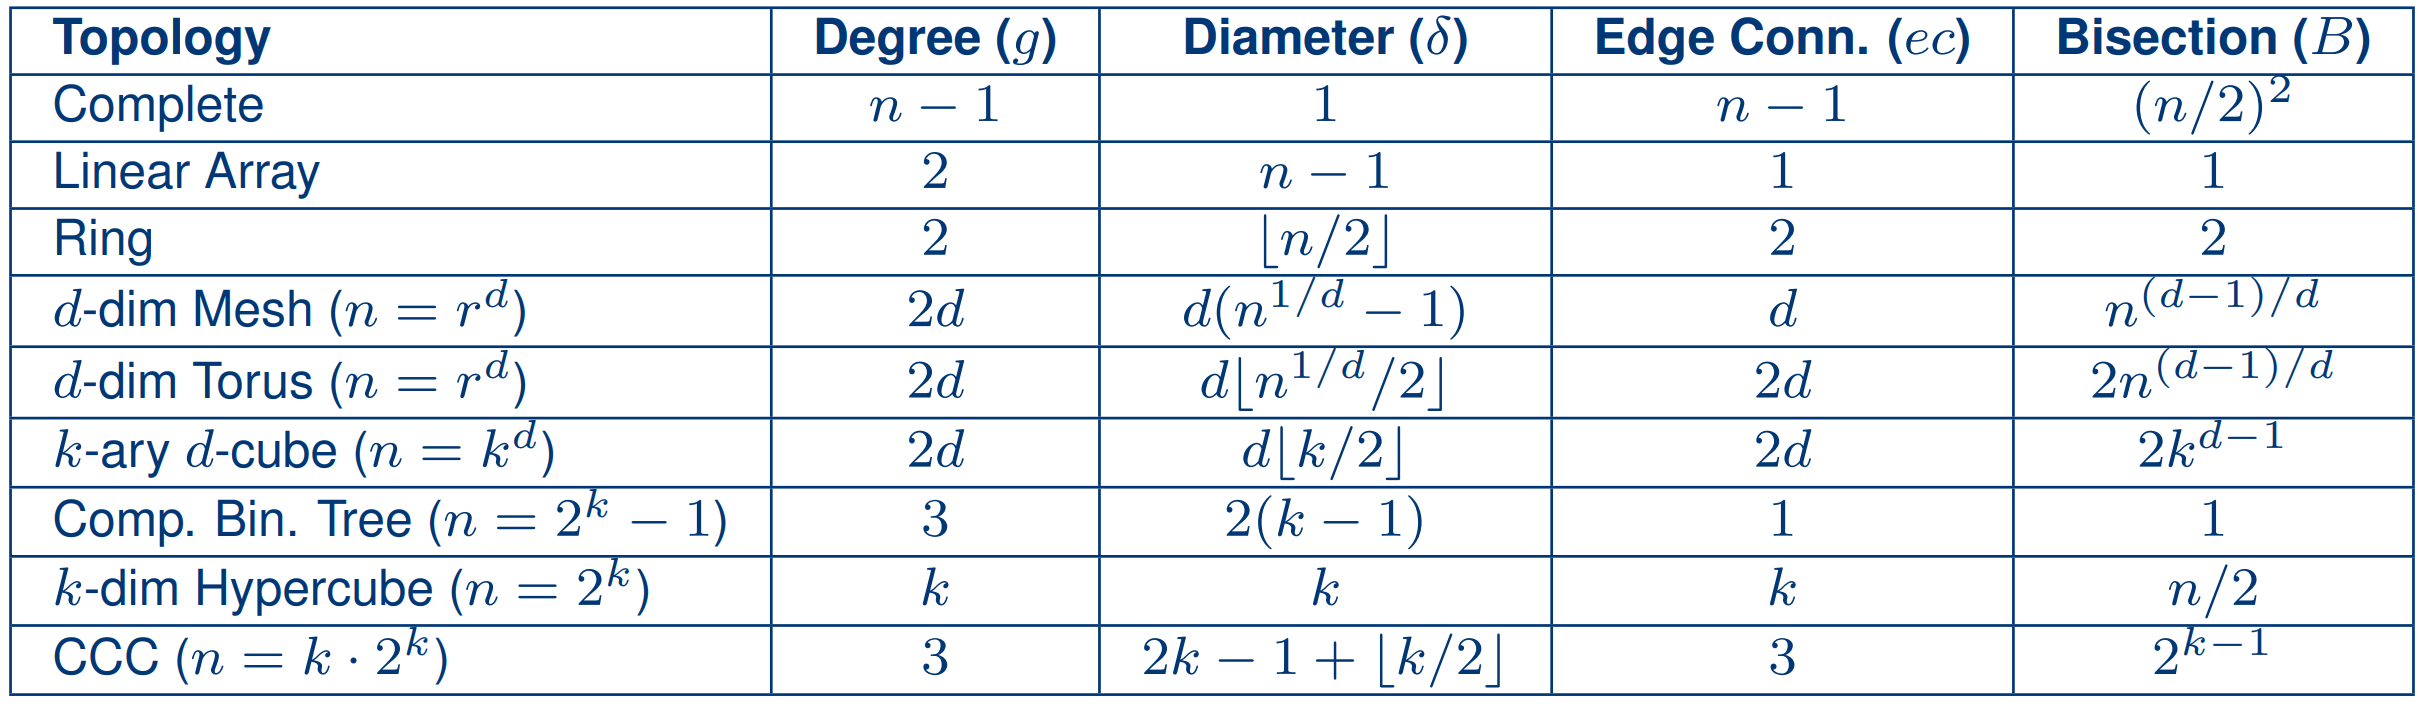
\includegraphics[width=1\linewidth]{topology.png}
\end{center}

\end{multicols*}

% \begin{minipage}{\textwidth}
%     \centering
%     \label{tab:network_topologies}
%     % resizebox handles the "too fat" problem by scaling it to the margins
%     \resizebox{\textwidth}{!}{
%         \begin{tabular}{|l|c|c|c|c|}
%         \hline
%         \textbf{Topology} & \textbf{Degree ($g$)} & \textbf{Diameter ($\delta$)} & \textbf{Edge Conn. ($ec$)} & \textbf{Bisection ($B$)} \\ \hline
%         Complete & $n - 1$ & $1$ & $n - 1$ & $(n/2)^2$ \\ \hline
%         Linear Array & $2$ & $n - 1$ & $1$ & $1$ \\ \hline
%         Ring & $2$ & $\lfloor n/2 \rfloor$ & $2$ & $2$ \\ \hline
%         $d$-dim Mesh ($n=r^d$) & $2d$ & $d(n^{1/d}-1)$ & $d$ & $n^{(d-1)/d}$ \\ \hline
%         $d$-dim Torus ($n=r^d$) & $2d$ & $d \lfloor n^{1/d}/2 \rfloor$ & $2d$ & $2n^{(d-1)/d}$ \\ \hline
%         $k$-ary $d$-cube ($n=k^d$) & $2d$ & $d \lfloor k/2 \rfloor$ & $2d$ & $2k^{d-1}$ \\ \hline
%         Comp. Bin. Tree ($n=2^k-1$) & $3$ & $2(k-1)$ & $1$ & $1$ \\ \hline
%         $k$-dim Hypercube ($n=2^k$) & $k$ & $k$ & $k$ & $n/2$ \\ \hline
%         CCC ($n = k \cdot 2^k$) & $3$ & $2k - 1 + \lfloor k/2 \rfloor$ & $3$ & $2^{k-1}$ \\ \hline
%         \end{tabular}
%     }
% \end{minipage}

\end{document}